%  This is free software: you can redistribute it and/or modify
%  it under the terms of the GNU General Public License as published by
%  the Free Software Foundation, either version 3 of the License, or
%  (at your option) any later version.
%
%  This is distributed in the hope that it will be useful,
%  but WITHOUT ANY WARRANTY; without even the implied warranty of
%  MERCHANTABILITY or FITNESS FOR A PARTICULAR PURPOSE.  See the
%  GNU General Public License for more details.
%
%  You can find the GNU General Public License at <http://www.gnu.org/licenses/>.
\documentclass[a0paper,portrait]{baposter}
%%%%%%%%%%%%%%%%%%%%%%%%%%%%%%%%%%%%%%%%%%%%%%%%
% Language, Encoding and Fonts
% http://en.wikibooks.org/wiki/LaTeX/Internationalization
%%%%%%%%%%%%%%%%%%%%%%%%%%%%%%%%%%%%%%%%%%%%%%%%
% Select encoding of your inputs. Depends on
% your operating system and its default input
% encoding. Typically, you should use
%   Linux  : utf8 (most modern Linux distributions)
%            latin1 
%   Windows: ansinew
%            latin1 (works in most cases)
%   Mac    : applemac
% Notice that you can manually change the input
% encoding of your files by selecting "save as"
% an select the desired input encoding. 
\usepackage[utf8]{inputenc}
% Make latex understand and use the typographic
% rules of the language used in the document.
\usepackage[english]{babel}
% Use the vector font Latin Modern which is going
% to be the default font in latex in the future.
\usepackage{helvet}
% Change the default font family from roman to sans serif
\renewcommand{\familydefault}{\sfdefault} % for text
\usepackage[helvet]{sfmath} % for math
% Choose the font encoding
\usepackage[T1]{fontenc}

%%%%%%%%%%%%%%%%%%%%%%%%%%%%%%%%%%%%%%%%%%%%%%%%
% Graphics and Tables
% http://en.wikibooks.org/wiki/LaTeX/Importing_Graphics
% http://en.wikibooks.org/wiki/LaTeX/Tables
% http://pgfplots.sourceforge.net/
%%%%%%%%%%%%%%%%%%%%%%%%%%%%%%%%%%%%%%%%%%%%%%%%
% You cannot use floats in the baposter theme.
% We therefore load the caption package which provides
% the command \captionof
% Set up how figure and table captions are displayed
\usepackage[skip=2pt]{caption}
\captionsetup{
  font=small,% set font size to footnotesize
  labelfont=bf % bold label (e.g., Figure 3.2) font
}
% Make the standard latex tables look so much better
\usepackage{array,booktabs}
% For creating beautiful plots
\usepackage{pgfplots}
% For SVG images
\usepackage{svg}
%%%%%%%%%%%%%%%%%%%%%%%%%%%%%%%%%%%%%%%%%%%%%%%%
% Mathematics
% http://en.wikibooks.org/wiki/LaTeX/Mathematics
%%%%%%%%%%%%%%%%%%%%%%%%%%%%%%%%%%%%%%%%%%%%%%%%
% Defines new environments such as equation,
% align and split 
\usepackage{amsmath}
% Adds new math symbols
\usepackage{amssymb}
% scaling etc
\usepackage{graphicx}

%%%%%%%%%%%%%%%%%%%%%%%%%%%%%%%%%%%%%%%%%%%%%%%%
% Colours
% http://en.wikibooks.org/wiki/LaTeX/Colors
%%%%%%%%%%%%%%%%%%%%%%%%%%%%%%%%%%%%%%%%%%%%%%%%
\selectcolormodel{RGB}
% define the three blue colors
\definecolor{nustblue}{RGB}{0,72,121}% dark blue
\definecolor{nustblue1}{RGB}{113,109,143} % light blue
\definecolor{nustblue2}{RGB}{194,193,204} % lighter blue
\definecolor{nustblue3}{RGB}{100,100,255}
%%%%%%%%%%%%%%%%%%%%%%%%%%%%%%%%%%%%%%%%%%%%%%%%
% Lists
% http://en.wikibooks.org/wiki/LaTeX/List_Structures
%%%%%%%%%%%%%%%%%%%%%%%%%%%%%%%%%%%%%%%%%%%%%%%%
% Easier configuration of lists
\usepackage{enumitem}
%configure itemize
\setlist{%
  topsep=0pt,% set space before and after list
  noitemsep,% remove space between items
  labelindent=\parindent,% set the label indentation to the paragraph indentation
  leftmargin=*,% remove the left margin
  font=\color{nustblue}\normalfont, %set the colour of all bullets, numbers and descriptions to nustblue
}
% use set<itemize,enumerate,description> if you have an older latex distribution
\setitemize[1]{label={\raise1.25pt\hbox{$\blacktriangleright$}}}
\setitemize[2]{label={\scriptsize\raise1.25pt\hbox{$\blacktriangleright$}}}
\setitemize[3]{label={\raise1.25pt\hbox{$\star$}}}
\setitemize[4]{label={-}}
%\setenumerate[1]{label={\theenumi.}}
%\setenumerate[2]{label={(\theenumii)}}
%\setenumerate[3]{label={\theenumiii.}}
%\setenumerate[4]{label={\theenumiv.}}
%\setdescription{font=\color{nustblue}\normalfont\bfseries}

% use setlist[<itemize,enumerate,description>,<level>] if you have a newer latex distribution
%\setlist[itemize,1]{label={\raise1.25pt\hbox{$\blacktriangleright$}}}
%\setlist[itemize,2]{label={\scriptsize\raise1.25pt\hbox{$\blacktriangleright$}}}
%\setlist[itemize,3]{label={\raise1.25pt\hbox{$\star$}}}
%\setlist[itemize,4]{label={-}}
%\setlist[enumerate,1]{label={\theenumi.}}
%\setlist[enumerate,2]{label={(\theenumii)}}
%\setlist[enumerate,3]{label={\theenumiii.}}
%\setlist[enumerate,4]{label={\theenumiv.}}
%\setlist[description]{font=\color{nustblue}\normalfont\bfseries}

%%%%%%%%%%%%%%%%%%%%%%%%%%%%%%%%%%%%%%%%%%%%%%%%
% Misc
%%%%%%%%%%%%%%%%%%%%%%%%%%%%%%%%%%%%%%%%%%%%%%%%
% change/remove some names
\addto{\captionsenglish}{
  %remove the title of the bibliograhpy
  \renewcommand{\refname}{\vspace{-0.7em}}
  %change Figure to Fig. in figure captions
  \renewcommand{\figurename}{Fig.}
}

\usepackage[style=ieee,backend=biber]{biblatex}
\AtEveryBibitem{\clearfield{note}\clearfield{url}}
\renewcommand{\bibname}{}
\renewcommand{\refname}{}
\addbibresource{ZotLibrary.bib}

% create links
\usepackage{url}
%note that the hyperref package is currently incompatible with the baposter class

%%%%%%%%%%%%%%%%%%%%%%%%%%%%%%%%%%%%%%%%%%%%%%%%
% Macros
%%%%%%%%%%%%%%%%%%%%%%%%%%%%%%%%%%%%%%%%%%%%%%%%
\newcommand{\alert}[1]{{\color{nustblue}#1}}

%%%%%%%%%%%%%%%%%%%%%%%%%%%%%%%%%%%%%%%%%%%%%%%%
% Document Start 
%%%%%%%%%%%%%%%%%%%%%%%%%%%%%%%%%%%%%%%%%%%%%%%%
\begin{document}
%%%%%%%%%%%%%%%%%%%%%%%%%%%%%%%%%%%%%%%%%%%%%%%%
% Some changes that cannot be made in the preamble
%%%%%%%%%%%%%%%%%%%%%%%%%%%%%%%%%%%%%%%%%%%%%%%%
% set the background of the poster
\background{
  \begin{tikzpicture}[remember picture,overlay]
    %the poster background color
    \fill[fill=nustblue2] (current page.north west) rectangle (current page.south east);
    %the header
    \fill [fill=nustblue] (current page.north west) rectangle ([yshift=-\headerheight] current page.north east);
  \end{tikzpicture}
}
% if you want to reduce the space before and after equations, use and adjust
% the following lines
\addtolength{\abovedisplayskip}{-2mm}
\addtolength{\belowdisplayskip}{-2mm}

%%%%%%%%%%%%%%%%%%%%%%%%%%%%%%%%%%%%%%%%%%%%%%%%
% General poster setup
%%%%%%%%%%%%%%%%%%%%%%%%%%%%%%%%%%%%%%%%%%%%%%%%
\begin{poster}{
  %general options for the poster
  grid=false,
  columns=3,
%  colspacing=4.2mm,
  headerheight=0.1\textheight,
  background=none,
%  bgColorOne=red!42, %is used when background != user and none
%  bgColortwo=green!42, %is used when background is shaded
  eyecatcher=true,
  %posterbox options
  headerborder=closed,
  borderColor=nustblue,
  headershape=rectangle,
  headershade=plain,
  headerColorOne=nustblue,
%  headerColortwo=yellow!42, %is used when the header background is shaded
  textborder=rectangle,
  boxshade=plain,
  boxColorOne=white,
%  boxColorTwo=cyan!42,%is used when the text background is shaded
  headerFontColor=white,
  headerfont=\Large\sf\bf,
  linewidth=1pt
}
%the Eye Catcher (the logo on the left)
{
  %this can be commented out or replaced by a company/department logo
  
\includegraphics[height=0.90\headerheight]{images/UoL_logo.png}
}
%the poster title
{\color{nustblue}\bf
    Nanomechanical Analysis of Renal Tubular 
    Cell Cytoskeleton to Measure Renal Disease
}
%the author(s)
{\small
  \vspace{1em} Joseph Ashton \quad SID 27047440 \qquad | \qquad Supervised by Eleftherios Siamantouras\\[0.5em]
  BEng (Hons) Mechatronics, School of Engineering and Physical Sciences, University of Lincoln\\
}
%the logo (the logo on the right)
{
  % 
\includegraphics[height=0.95\headerheight]{images/SDG_TARGET_34.png}
  \includesvg[height=\headerheight]{images/SDG_TARGET_34.svg}
}

%%%%%%%%%%%%%%%%%%%%%%%%%%%%%%%%%%%%%%%%%%%%%%%%
% the actual content of the poster begins here
%%%%%%%%%%%%%%%%%%%%%%%%%%%%%%%%%%%%%%%%%%%%%%%%

\begin{posterbox}[name=abstract,column=0,row=0]{Abstract}
\begin{justify}
    This project investigates changes in mechanical properties of kidney
    cells when exposed to TGF-\(\beta 1\), which is known to induce
    renal disease \cite{gentleME2013-EpithelialCellTGFv}. The aim of this project is to provide insight
    on the progression of diabetic nephropathy from a mechanical
    perspective based on changes in mechanical properties observed in
    single cells using atomic force microscopy.
\end{justify}
\end{posterbox}

\begin{posterbox}[name=equations,column=0,below=abstract,above=recommend]{Equations}
\begin{small}

\begin{equation}
  F(\delta) = \frac{4}{3} \cdot \frac{E}{1 - \nu^2} \cdot \sqrt{R} \cdot \delta^{3/2}
  \label{eq:hertz}
\end{equation} 

\vspace{5pt}

\begin{minipage}[t]{0.575\linewidth}
  \vspace{0pt}

\begin{description}
  The Hertz/Sneddon spherical indentation model (Eq.~\ref{eq:hertz}) is matched to the force indentation curve to find the apparent elasticity of an experiment.
\end{description}

\end{minipage}
\hfill
\begin{minipage}[t]{0.2\linewidth}
  \vspace{-20pt}
\begin{align*}
  F & \text{::Force}\\
  E & \text{::Young's Modulus}\\
  v & \text{::Poisson's Ratio}\\
  R & \text{::Indenter Radius}\\
  \delta & \text{::Indentation depth}\\
\end{align*}
\end{minipage}
\vspace{-10pt}

\begin{equation}
  \hat{P}(G_2 \mid x) = \frac{P(x \mid G_2) \cdot P(G_2)}{P(x \mid G_1) \cdot P(G_1) + P(x \mid G_2) \cdot P(G_2)}
  \label{eq:classifier}
\end{equation} 

\begin{minipage}[t]{0.575\linewidth}
  \vspace{0pt}
  \begin{description}
    The Bayesian classifier is a function based on Bayes theorem that finds a posterior probability (the probability of a precondition given the result).
  \end{description}
\end{minipage}
\hfill
\begin{minipage}[t]{0.35\linewidth}
  \vspace{-10pt}
  \begin{align*}  
  P(G \mid x) & \text{::Posterior}\\
  P(x \mid G) & \text{::Likleyhood}\\
  P(G)        & \text{::Prior}\\
  P(x)        & \text{::Evidence}\\
  \end{align*}
\end{minipage}

\begin{description}
  Where the likelihood of a given group is determined by fitting the observed occurrences to a distribution / Probability Density Function (PDF). 
  3 distribution models are tested:
  Gaussian (Eq.~\ref{eq:gaussian}),  
  Skewed Normal (Eq.~\ref{eq:skewnorm}), and  
  Kernel Density Estimation (Eq.~\ref{eq:kde}).
\end{description}

\begin{equation}
  \hat{P}(x \mid G) =  
  \frac{1}{\sigma_{G} \sqrt{2 \pi}}  
  e^{\tfrac{-1}{2}  
  \left( \tfrac{x-\mu_{G}}{\sigma_{G}}\right)^{2}}  
  \label{eq:gaussian}
\end{equation}

\begin{equation}
  \hat{P}(x \mid G) =  
  \phi\left(x; \mu_G, \sigma_G \right)
  \cdot  
  \Phi\left(  
  \alpha_G \cdot \frac{x - \mu_G}{\sigma_G}  
  \right)
  \label{eq:skewnorm}
\end{equation}

\begin{equation}
  \hat{P}(x \mid G) =  
  \frac{1}{n h} \sum_{i=1}^{n} K\left( \frac{x - x_{i_G}}{h} \right)  
  \label{eq:kde}
\end{equation}

\begin{align*}
  \hat{P}(x \mid G)     &:: \text{Group Probability Density Function}\\
  x                     &:: \text{Observation (i.e. Young's Modulus)}\\
  \sigma_{G}            &:: \text{Group Standard Deviation}\\
  \mu_{G}               &:: \text{Group Mean}\\
  \phi(x; \mu, \sigma)  &:: \text{Normal PDF evaluated at } x \\
  \alpha_G              &:: \text{Group Skew Parameter} \\
  \Phi(z)               &:: \text{Standard Normal CDF} \\
  x_{i_G}               &:: \text{Observed Data Points from Group G}\\
  n                     &:: \text{Number of Observations}\\
  K(\cdot)              &:: \text{Kernel Function (i.e. Gaussian)}\\
  h                     &:: \text{Bandwidth (Smoothing Parameter)}\\
\end{align*}
\end{small}

\end{posterbox}

\begin{posterbox}[name=recommend,column=0,below=equations,above=bottom]{Recommendations}
  \begin{description}
    \item [Repeat with larger experimental dataset] Applying the methodology described on larger datasets would allow for a more robust estimate with more extensive testing and validation.
  \end{description}
\end{posterbox}

\begin{posterbox}[name=intro,span=2,column=1,row=0]{Introduction}
This project investigates the predictive power of renal tubular epithelial cell stiffness as a biomarker for the progression of Diabetic Nephropathy (DN). 
DN is a common and serious complication of diabetes resulting in kidney failure due to progressive damage to the nephrons, the functional units of the kidney responsible for filtering the blood \cite{metcalfeW2007-HowDoesEarlyChronicKidneyDiseaseProgress}.
This loss of function is due to physical changes at the cellular level induced by cytokine TGF-$\beta$ 1 associated with an observable change in cytoskeleton stiffness \cite{hillsCE2012-TGFvModulatesCelltocell}. 

\begin{minipage}[t]{0.775\linewidth}
  \vspace{0pt}
  A force against indentation curve of a cells can be observed using Atomic Force Microscopy (AFM) where the deflection of a very fine probe on a flexible cantilever is measured to detect contact forces. 
  From the spring constant of the cantilever the indentation and force exerted can be determined as the assembly is advanced into the sample. 
  This curve can then be fitted against an elastic deformation model to determine an apparent Young's Modulus (YM). 
\end{minipage}
\hfill
\begin{minipage}[t]{0.2\linewidth}
  \vspace{-10pt}
  \centering
  % 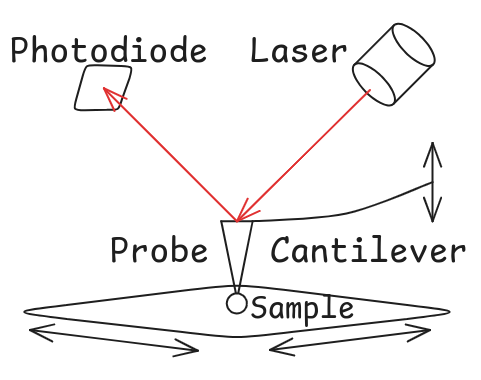
\includegraphics[width=\linewidth]{images/Atomic Force Microscopy - mechanism diagram.png}
  \includesvg[width=\linewidth,textsize=2pt]{images/Atomic Force Microscopy - mechanism diagram.svg}
  \captionof{figure}{AFM Diagram}
\end{minipage}
\vspace{1em}

The probability a given cell is healthy or diseased can be predicted from the observed distributions of YM of cells that have not been exposed to TGF-$\beta$ (Control) and those that have (Treated) by a Bayesian classifier.

\end{posterbox}


\begin{posterbox}[name=method,span=2,column=1,below=intro]{Methodology}
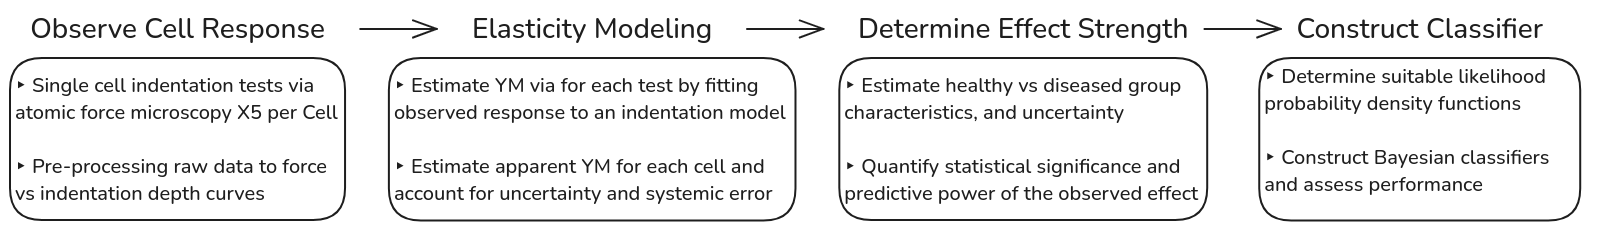
\includegraphics[width=\linewidth]{images/Methodology Summary Blocks.png}

\end{posterbox}

\begin{posterbox}[name=results,column=1,below=method,above=bottom]{Results}
  
\begin{center}
\end{center}

\end{posterbox}

\begin{posterbox}[name=discuss,column=2,below=method]{Discussion}
  \begin{items}
    \item Applying the methodology described on larger datasets would allow for a more robust estimate with more extensive testing and validation.
  \end{items}
\end{posterbox}

\begin{posterbox}[name=refs,column=2,below=discuss,above=bottom]{References}
  \defbibheading{none}{}  % remove redundant heading
  \renewcommand*{\bibfont}{\scriptsize}
  \printbibliography[heading=none]
\end{posterbox}

\end{poster}
\end{document}
